\documentclass[a4paper,11pt,fleqn]{article}%fleqn pour aligner les equations à gauche
\usepackage{../../Styles/Exercice}


\newcommand{\chnum}{Chapitre 12}
\newcommand{\chtitle}{Modélisation d'un fluide au repos}
\newcommand{\dtype}{Exercices}

\begin{document}
	\maketitle
\begin{multicols}{2}
\section{Schématiser une force pressante}
Représenter la force pressante qu’exerce une solution sur la paroi du fond d’un bécher, sans soucis d’échelle.

\section{Interpréter un schéma}
Un aquarium est rempli d’eau. Que représente le vecteur $\vec{F}$ sur le dessin ?
\begin{center}
	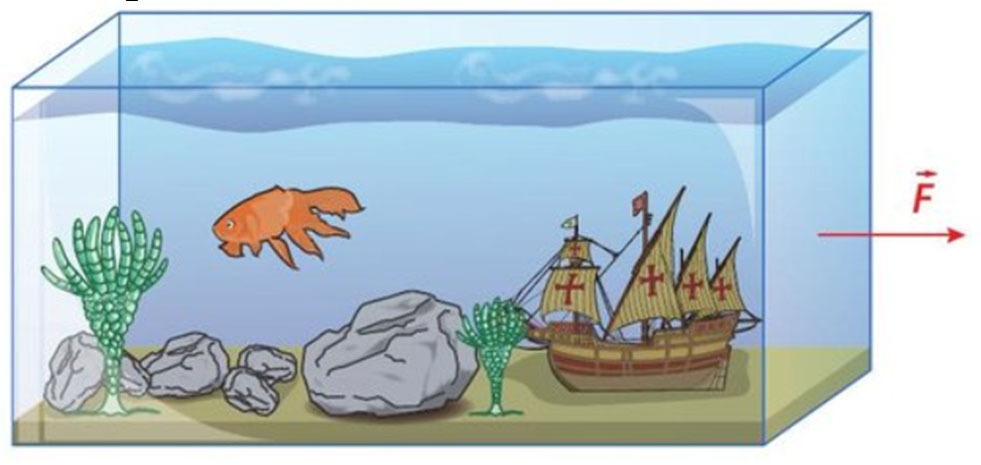
\includegraphics[width=.5\linewidth]{Ressources/1SPE_C12_Ex_Fig1.png}
\end{center}

\section{Calculer la valeur d'une force pressante}
Les deux faces d’une palissade de jardin ont chacune une surface notée $S$. La pression atmosphérique est notée
$P$. Calculer la valeur $F$ de la force pressante exercée par l’air sur chaque face de cette palissade.
\begin{data}
$S=\SI{15E2}{\meter\squared}$\\
$P_{atm} = \SI{1,013E5}{\pascal}$
\end{data}

\section{Calculer une pression}
Une skieuse se trouve en haut de la piste de ski lors des Jeux Olympiques de 2018 à Pyeongchang. Elle porte un
masque de surface $S = \SI{1,3E-2}{\meter\squared}$. la force pressante excercée par l'air extérieur sur le masque vaut $F = \SI{1,2E3}{\newton}$. Calculer la pression atmosphérique $P_{atm}$ en haut de la piste.

\section{Tension artérielle}
On appelle tension (ou pression) artérielle $T$ la différence entre la pression du sang et la pression atmosphérique :
$$T = P_{sang}-P_{atm}$$
Lors d’un examen médical, le médecin annonce deux valeurs de tension artérielle :
\begin{itemize}
	\item La pression maximale (ou pression systolique) qui correspond à la pression du sang au moment de la
	contraction du cœur
	\item La pression minimale (ou pression diastolique) qui correspond au relâchement du cœur.
\end{itemize}
Ces valeurs sont données dans une unité particulière qui est le centimètre de mercure (\unit{cm~Hg}).
Pendant un contrôle médical, un médecin annonce à un sportif une tension de « 12-8 ».
\begin{enumerate}
	\item Exprimer les deux tensions artérielles en pascal.
	\item Calculer la pression du sang  pour ces deux valeurs.
\end{enumerate}
\begin{data}
	\SI{1}{cm~Hg} correspond à \SI{1333}{\pascal}\\
	$P_{atm} = \SI{1,013E5}{\pascal}$
\end{data}



\section{Assurer l'eau courante pour tous}
Pour assurer une distribution correcte de l'eau courante, la pression $P_1-P_2$ au niveau d'un robinet fermé doit être de \SI{3,0}{\bar}. Lors de la construction d'un écoquartier sur un terrain plat, on souhaite fabriquer un château d'eau de hauteur $h_2$ permettant d'assurer la distribution à un immeuble dont le dernier étage se situe à une hauteur $h_1 = \SI{10}{m}$.
\begin{enumerate}
	\item Réaliser un schéma de la situation mettant en évidence les hauteur $h_1$ et $h_2$.
	\item Exprimer et calculer la hauteur minimale $h_2$ du château d'eau permettant d'assurer une distribution correcte d'eau courante au dernier étage de l'immeuble.
\end{enumerate}
\begin{data}
	Pression Atmosphérique : $P_{atm} = P_2 = \SI{1,0}{\bar} = \SI{1,0E5}{\pascal}$
\end{data}
\section{Remplir les cartouches d'un siphon à chantilly}
En pâtisserie, un siphon permet de réaliser des crèmes chantilly bien aérées. Les cartouches de gaz d’un tel siphon contiennent \SI{8,0}{g} de protoxyde d’azote \ce{N2O}. Cette masse correspond à un volume $V_1 = \SI{4,4}{L}$ de gaz quand la pression atmosphérique est $P_1 = \SI{1,0}{\bar}$ et la température $\theta_1 = \SI{20}{\celsius}$. La notice de la cartouche indique que la pression à l'intérieur de la cartouche est $P_2 = \SI{71}{\bar}$.
\begin{enumerate}
	\item Calculer la masse volumique $\rho$ du protoxyde d'azote à la pression $P_1$ et à la température $\theta_1$.
	\item Exprimer et calculer le volume $V_2$ occupé par \SI{8}{g} de protoxyde d'azote gazeux \ce{N2O} à la température $\theta_1$ et à  la pression à l’intérieur de la cartouche $P_2$.
	\item Exprimer et calculer la capacité, c'est-à-dire le volume, de la cartouche, notée $V_C$, si le siphon  est assimilé à un cylindre de hauteur $h = \SI{6,5}{cm}$ et de diamètre $D=\SI{1,8}{cm}$.
	\item Relever l'incohérence de ces deux résultats et proposer une explication.
	
\end{enumerate}
\end{multicols}
\end{document}